% LaTeX2e Template by Stephen Iota (https://stepheniota.github.io/)
% last updated: Oct. 2018

% for papers
%\documentclass[aps,onecolumn,superscriptaddress]{revtex4-1}
% https://www-d0.fnal.gov/Run2Physics/WWW/templates/revtex4.pdf
% https://cdn.journals.aps.org/files/revtex/auguide4-1.pdf
% for revTeX4-1 class options

% for other
\documentclass[12pt]{article}
\usepackage[margin=2cm]{geometry}

%%%%%%%%%%%%%%%%
%%% Packages %%%
%%%%%%%%%%%%%%%%

\usepackage[utf8]{inputenc}
\usepackage{amsmath}
\usepackage{amssymb}
\usepackage{amsfonts} % to remove math font when typesetting equations
\usepackage{graphicx}
\usepackage[shortlabels]{enumitem} % to change labels in enum/item
\usepackage[dvipsnames]{xcolor} % for colored links


% always put this at the end
\usepackage[
	colorlinks=true,
	citecolor=green!50!black,
	linkcolor=NavyBlue!75!black,
	urlcolor=green!50!black,
	hypertexnames=false]{hyperref} 

 
 %%%%%%%%%%%%%%%%%%
 %% New Commands %%
 %%%%%%%%%%%%%%%%%%
 
\newcommand{\email}[1]{\texttt{\href{mailto:#1}{#1}}}

\newcommand{\hint}[1]{\color{Blue}{#1}}
 
%----------------------------------------------------
%%%%%%%%%%%%%%%%%%
%% Front Matter %%
%%%%%%%%%%%%%%%%%%

%\pagenumbering{gobble} % no page numbers
\graphicspath{{figures/}} % set directory for figures
\usepackage{wrapfig}
\setcounter{section}{-1} % start with section 0

%%%%%%%%%%%%%
%%% Title %%%
%%%%%%%%%%%%%
\begin{document}

\begin{center}

\Large{\textsc{Worksheet 4}: \textbf{Connecting $V$ and $\vec{E}$}}

\end{center}

\vspace{.5mm}

%%%%%%%%%%
%% INFO %%
%%%%%%%%%%

\begin{tabular}{rl}
\textsc{SI Leader}:
&
Stephen Iota (\email{siota001@ucr.edu})
\\
\textsc{Course}:
&
Physics 40C (Fall 2018), Dr.~Laura Sales
\\
\textsc{Date}:
&
25 October 2018
\end{tabular}

%%%%%%%%%%%%%%
%% PROBLEMS %%
%%%%%%%%%%%%%%

\section{Comments}
Slightly fewer problems this week.
The goal is to focus more on problem solving skills, trying to understand each step at a deep level when going through a solution.

\section{Kirchhoff's Loop Law}
Kirchhoff's Loop Law states the sum of all potential differences encountered while moving around a closed loop is zero.
$$ \Delta V_\mathrm{loop} = \sum_i (\Delta V)_i = 0 $$
Prove that this is just a statement of conservation of energy.\footnote{In other words, this law doesn't tell us anything we didn't know from 40A.}

\vspace{32mm}
\section{Parallel-Plate Capacitor}
Earlier in the quarter, we learned that the electric field inside a parallel-plate capacitor is:
$$ \vec{E} = \Bigg(\frac{Q}{\epsilon_0 A},+\rightarrow-\Bigg) $$
Let $ V = 0 $ at the negative plate.
Find the \textbf{electric potential} inside the capacitor. 


\newpage

\section{Capacitance}

The figure below shows two electrodes charged to $\pm Q$. Although net charge is equal to zero, there is a potential difference $\Delta V$ between the electrodes. We define \textbf{capacitance} $C$ to be the proportionality constant that relates charge\footnote{Here, $Q$ refers to the magnitude of the charge on \emph{one} of the electrodes. The electrodes of a capacitor always have \emph{equal but opposite} charges.  } to potential.
$$ Q = C \Delta V_C  \ \ \ \ \ \  (\text{charge on a capacitor}) $$
% there's gotta be a better way to put text into an equation, but i'm in a pinch! 

\noindent
Prove that capacitance \textbf{depends only on the geometry of the electrodes}.
\begin{center}
	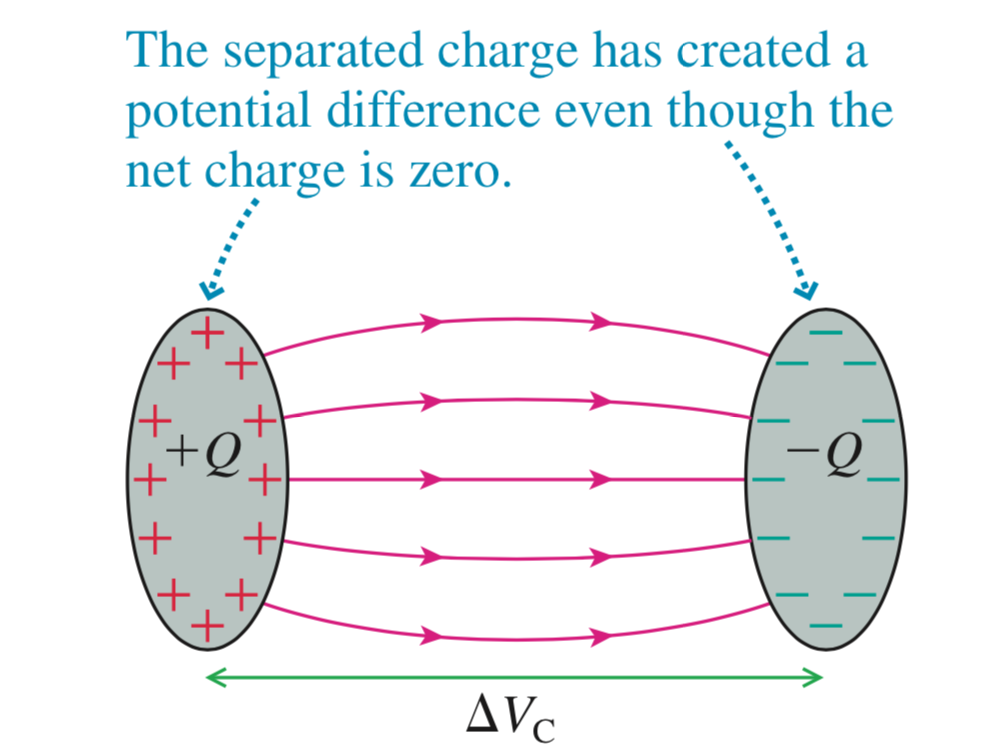
\includegraphics[width=.3\linewidth]{W4_f1}
\end{center}



\end{document}